\chapter{Analiza tematu}

W niniejszym opracowaniu zostaną przedstawione zagadnienia związane z~renderowaniem scen z wykorzystaniem metody ray marching oraz techniką tworzenia proceduralnie generowanego terenu.

Rozwiązania tego typu mogą być wykorzystywane w~obszarach związanych z~tworzeniem filmów, gier komputerowych, animacji itp. Ta metoda renderowania na dzień dzisiejszy nie jest jeszcze zbyt powszechna, a przynajmniej nie w takim stopniu jak metody oparte o rasteryzację trójkątów czy ray tracing.

Biorąc pod uwagę sposób działania technik renderowania opartych o wiązki światła, przedstawienie generowanego terenu wykorzystując siatkę trójkątów nie jest wydajnym rozwiązaniem. Wiąże się to z ilością obliczeń koniecznych do wykrycia kolizji z każdym trójkątem siatki dla każdej wiązki światła. Znacznie lepszym  i wydajniejszym rozwiązaniem jest przedstawienie terenu jako (dwu argumentowej) funkcji matematycznej.

Do kształtowania terenu w pierwszej kolejności zostanie wykorzystana funkcja zwracająca pseudolosową wartość dla danego dwuwymiarowego punktu.
W tym celu można użyć z wielu różnych metod, przykładowo wykorzystując dwuwymiarową teksturę
lub funkcję matematyczną której wyniki przypominają losowe wartości. Aby uzyskać ciągłą funkcję, wartość każdego punktu jest interpolowana na podstawie czterech najbliższych punktów, których współrzędne są wartościami całkowitymi.

Aby uzyskać porządany efekt zaimplementowana została interpolacja biliniowa opisana wzorem \ref{eq:interp-biliniowa}, dla wybranych punktów $a, b, c$ i $d$. Jako parametry tej funkcji $x$ i $y$ należą do przedziału $x, y \in [0, 1]$. Przykład tego typu (może jakoś inaczej) interpolacji przedstawia rysunek \ref{fig:lerp}.
\begin{equation}
\label{eq:interp-biliniowa}
  \begin{split}
    f(x, y) & = a \\
       & + (b - a) * x \\
       & + (c - a) * y \\
       & + (a - b - c + d) * x * y
    \end{split}
\end{equation}

Można zauważyć, że efektem tej interpolacji są bardzo widoczne granice między grupami punktów, co przedstawia rysunek \ref{z programu}.

Rozwiązaniem tego problemu jest zastosowanie funkcji \ang{smoothstep} pozwalającej na uzyskanie wygładzonej interpolacji. W tym celu zmodyfikowano wzór \ref{eq:interp-biliniowa}, zastępując parametry $x$ i $y$ wykorzystując funkcję \ang{smoothstep} $n$-tego stopnia przedstawionej jako $S_n(p)$. Ostateczną postać funkcji przedstawia wzór \ref{eq:smooth-interp}. Obliczając gradient tej funkcji, można zauważyć, że wartości pochodnej dla każdego z czterech granicznych punktów jest równa $0$, dzięki czemu przejścia między grupami punktów nie są widoczne.

\begin{equation}
\label{eq:smooth-interp}
  \begin{split}
    f(x, y) & = a \\
       & + (b - a) * S_n(x) \\
       & + (c - a) * S_n(y) \\
       & + (a - b - c + d) * S_n(x) * S_n(y)
    \end{split}
\end{equation}

W programie wykorzystana została funkcja \ang{smoothstep} pierwszego stopnia, której postać jest widoczna na wzorze \ref{eq:smooth-interp-1}.

\begin{equation}
\label{eq:smooth-interp-1}
  \begin{split}
    S_1(x) = 3x^2 - 2x^3
  \end{split}
\end{equation}

Wynik zastosowania tego wzoru ukazuje rysunek \ref{fig:smooth-interp}.


\begin{figure}
\centering
\subfloat[interpolacja biliniowa]{
  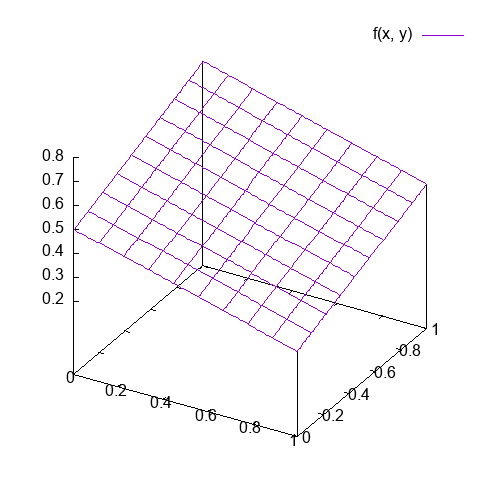
\includegraphics[width=0.5\textwidth]{./graf/plot/bilinear.png}
  \label{fig:lerp}
}
\subfloat[interpolacja wykorzystujące funkcję \ang{smoothstep} pierwszego stopnia]{
  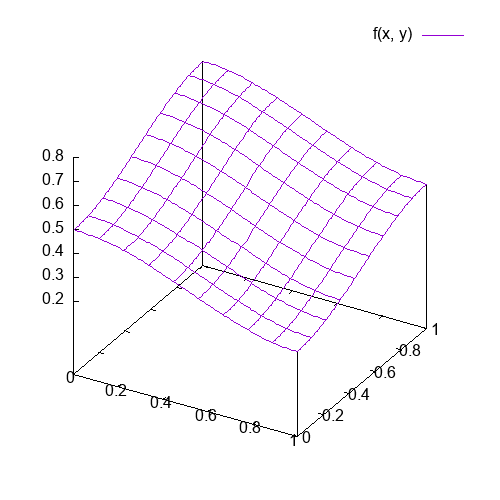
\includegraphics[width=0.5\textwidth]{./graf/plot/smooth.png}
  \label{fig:smooth-interp}
}
%% 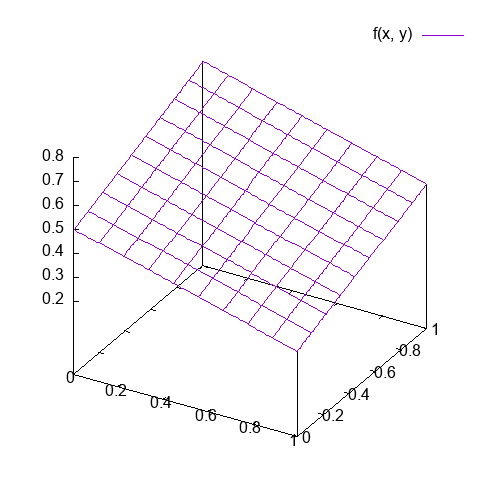
\includegraphics[width=0.65\textwidth]{./graf/plot/bilinear.png}
\caption{Porównanie wyników obu metod interpolacji między czterema punktami}
\label{fig:interpolacja}
\end{figure}


%% \begin{itemize}
%% \item sformułowanie problemu
%% \item osadzenie tematu w kontekście aktualnego stanu wiedzy (\ang{state of the art}) o poruszanym problemie
%% \item  studia literaturowe \cite{bib:artykul,bib:ksiazka,bib:konferencja,bib:internet} -  opis znanych rozwiązań (także opisanych naukowo, jeżeli problem jest poruszany w publikacjach naukowych), algorytmów,
%% \end{itemize}


%% Wzory
%% \begin{align}
%% y = \frac{\partial x}{\partial t}
%% \end{align}
%% jak i pojedyncze symbole $x$ i $y$  składa się w trybie matematycznym.
